\subsection{Process for Manufacturing of Polymer Matrix Composites}
\subsubsection{Assembly of Laminate}
When constructing composite materials, the direction of the graphite fibers within the epoxy resin matrix directly impact the material's structural properties.  To later test the differences in structural properties, three directional laminates are constructed as (a): $[90\degree]_{16\text{T}}$, (b): $[\pm45\degree_4]_{2\text{S}}$, and (c): $[0\degree]_{8\text{T}}$.  The three types of specimen are portrayed in Figure \ref{fig:specconfig}.

\begin{figure}[!h]
    \centering
    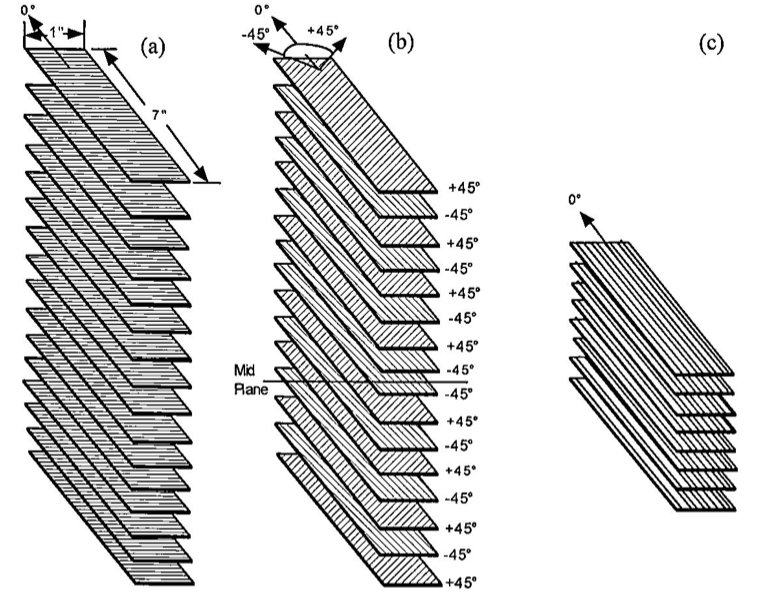
\includegraphics[width=0.65\textwidth]{Pictures/Procedure/specconfig.png}
    \caption{Specimen Configurations\cite{labmanual}}
    \label{fig:specconfig}
\end{figure}

In order to get these fiber configurations, the provided prepreg material is sliced using a razor knife and a cutting template into $1" x 7"$ strips.  As the prepreg strips are highly prone to premature curing at room temperature, the strips are placed in a cold location in the room to chill.  Per the teaching assistant's instructions, only eight strips are sliced of specimen (a) and (c) in contrast to the lab manual's instructed 16 slices for specimen (a).  When eight slices of (a), (c), and 16 slices of (b) are cut, the laminate may be assembled in accordance to Figure \ref{fig:specconfig} above to form three unique specimen.  After weighing and measuring the dimensions of the laminates, the three composite laminates are then ready for the lay-up process.

\subsubsection{Lay-up Procedure}
The lay-up process is very similar among each specimen.  First, the 2024-T3 Aluminium mold is prepared by spraying a lubricating aerosol in the mold slits and the spacer tools.  Then the stacking is set up as shown in Figure \ref{fig:stacking} in the order of release film, bleeder ply, peel ply, laminate, peel ply, bleeder ply, and release film.

\begin{figure}[!h]
    \centering
    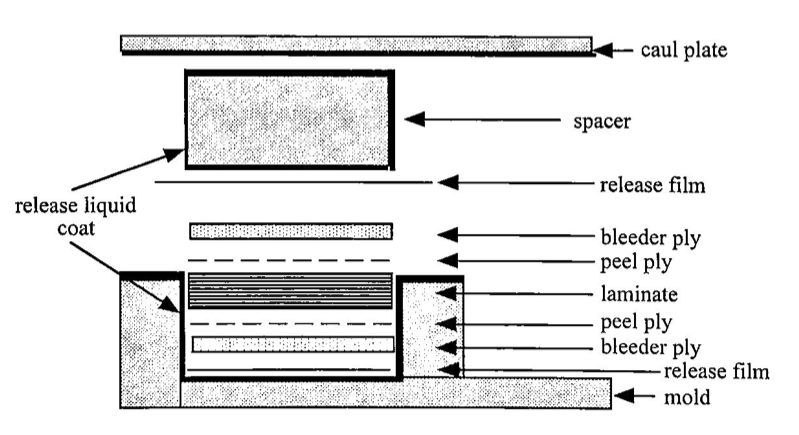
\includegraphics[width=0.85\textwidth]{Pictures/Procedure/lay-up.png}
    \caption{Lay-up Stacking Order \cite{labmanual}}
    \label{fig:stacking}
\end{figure}

Mentioned in greater detail in Table \ref{tab:equipmentpart1}, the bleeder cloth, peel ply, and release film all serve important roles in the curing process and must be placed in the correct order.  Throughout the lay-up procedure, whenever the specimen are placed into or around the mold, it is important to spray the mold frequently with lubricant to prevent any undesired adhesion between the specimen and mold.  When the specimen are placed into the mold, the aluminium spacer is lubricated and placed into the mold.  If necessary, a soft mallet may be used to drive the spacer and composite deeper into the mold.  With all three specimen and spacers in the mold, it is time to place the mold into the Carver programmable hot press for the thermosetting cure process.
\clearpage
\subsubsection{Curing Procedure}
Due to the dangerous nature of the curing process and the expensive machinery, the teaching assistants took the responsibility of curing the composites.  Without controlling the hot press machine, the exact programmed temperature and pressure applied at various time steps is not known.  The curing process, according to the lab manual, for materials such as DA 409U/G35 150 prepreg looks similar to Figure \ref{fig:mariecuring}.

\begin{figure}[!h]
    \centering
    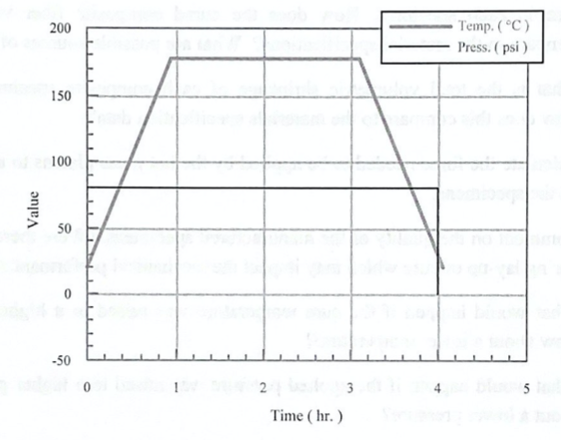
\includegraphics[width=0.65\textwidth]{Pictures/Procedure/mariecuring.png}
    \caption{Curing Cycle for DA 409U/G35 150 Prepreg \cite{labmanual}}
    \label{fig:mariecuring}
\end{figure}

Additional research into the use of a hot press for the curing process reveals significant mechanical and structural property variation depending on the temperature and pressure applied \cite{curematters}.  Therefore, for a proper cure of the material, the hot press must apply the precise temperature and pressure on the composites at certain time intervals to ensure proper thermosetting of the materials.

\clearpage
\subsection{Process for Mechanical Property Testing of Composite Materials}
\subsubsection{Specimen Geometry}


\subsubsection{Tension Test}